% !Mode:: "TeX:UTF-8"

\chapter{基于RISC-V的操作系统整体设计}[overall]
\label{chapter:overall}

\section{RISC-V相关硬件机制}

本节将简要介绍RISC-V规范中所规定的相关机制,主要聚焦于中断处理和内存管理,这两部分尤其需要硬件与软件配合,所以了解其硬件机制对于实现操作系统的相关模块尤为重要。

本节及其后的内容将基于RV64I,这是一个RISC-V最基础的64位整数指令集模块,也是RISC-V标准最先确定下来的部分。

\subsection{RISC-V特权模式}

RISC-V规范规定了三种特权模式,在任何时候,RISC-V架构上运行的线程都一定位于其中一种特权模式中。这些特权模式由多个控制寄存器(CSR)编码表示。RV64I标准定义的三个特权模式如表\ref{tab:privilege}。

\begin{table}[h]
	\centering
	\setlength{\belowcaptionskip}{2pt}
	\caption{RISC-V的三种特权模式}
	\label{tab:privilege}
	\begin{tabular}{cccc}
		\hline
		等级 & 编码 & 名称                          & 简写 \\ \hline
		0  & 00 & 用户/应用程序模式(User/Application) & U  \\ 
		1  & 01 & 监管者模式(Supervisor)           & S  \\ 
		2  & 10 & 未定义                         &    \\ 
		3  & 11 & 机器模式(Machine)               & M  \\ \hline
	\end{tabular}
\end{table}

如果当前指令试图执行当前特权模式不允许的操作,将引发异常。这些异常通常会导致自陷以进入下层执行环境进行处理。

所有的硬件实现都必须提供M-Mode,因为这是唯一可以自由访问整个机器的模式。最简单的RISC-V系统实现可能只提供M-Mode,但这种实现不会对系统提供保护以防止错误或是恶意的应用程序代码。通常,一个类Unix系统通常将M-Mode作为Bootloader的运行模式,需要实现S-Mode作为操作系统的主要运行模式,并对软件提供U-Mode的运行环境。

\subsection{RISC-V中断机制}
\label{sec:interrupt}

RISC-V中,能引起CPU从低权限特权级向高权限特权级转移的方式只有一种,那就是通过中断。

微观上,异常这个词表示当前硬件线程中执行代码发生的特殊情况,而中断则表示一个外部的异步事件,这个事件可能引起控制转移,通常与当前执行代码无关。宏观上,上述两种情况统称为中断。

RISC-V架构通过mstatus中的三个权限位管理全局的中断使能,分别是MIE、SIE和UIE。当硬件线程以x-Mode运行时,设置xIE位会启用全局中断响应,启用全局中断响应意味着,在该模式下运行的线程会被中断打断,并进入到中断处理流程中。

为了细化中断粒度,RISC-V启用了另一对寄存器:mip与mie。规范将RISC-V中断分为三种,分别是定时器中断、软件中断和外部中断。定时器中断是由外部定时器(通常位于主板上)定时向CPU引脚发送中断信号引发的,软件中断是由正在执行的程序主动自陷导致,而外部中断,则是由外部设备(如键盘等设备)向CPU发送中断信号导致,通常是向CPU请求处理外部状况。只有mip和mie寄存器中的位i(i 指时钟、软件或外部中断)被设置为1,且全局启用了中断,CPU才能响应i中断。

当一个中断发生时,如果开启了对应类别的中断,并且全局使能中断,那么当前硬件线程的执行流程会被打断,控制转移到中断处理程序。mtvec寄存器配置控制转移过程,该寄存器由一个向量基地址(BASE)和向量模式(MODE)组成。MODE模式决定了CPU如何按照BASE的值进行跳转,如表\ref{tab:mtvec}。

\begin{table}[h]
	\centering
	\setlength{\belowcaptionskip}{2pt}
	\caption{mtvec中MODE字段}
	\label{tab:mtvec}
	\begin{tabular}{ccc}
		\hline
		MODE             & 名称       & 描述                                        \\ \hline
		0                & Direct   & 所有中断发生时,都会跳转到BASE处                        \\
		1                & Vectored & 中断发生时,跳转到BASE+4*xcause中所保存的地址处 \\
		\textgreater{}=2 & —        & —                                         \\ \hline
	\end{tabular}
\end{table}

在中断处理结束后,可以通过xRET指令从中断处理中返回。当执行xRET指令后,控制会跳转到xepc寄存器中的地址处。进入中断之前的特权模式会被自动写入 sstatus寄存器的xPP位,于是xRET指令退出中断时也会根据xPP位恢复进入中断前的特权模式。我们可以借助这种机制,修改xPP位来完成从高权限特权级向低权限特权级的转换。

\subsection{RISC-V内存管理}

RISC-V采用分页机制来对内存进行管理。RISC-V中,一页是连续的4K字节(和大多数平台一致)。RISC-V中设置了三种分页模式来应对不同场景下的内存管理需求,实现时只需要根据平台特性选择一种即可。

RISC-V规范要求虚拟地址空间实现在S-Mode中,所以地址翻译相关的寄存器只有S-Mode视图的版本。其中,satp寄存器控制了地址翻译和保护。satp被划分为三个字段,其中,MODE字段用来开启分页并选择分页系统,PPN字段是根页表的物理页号。MODE字段可选编码如表\ref{tab:satpmode}。

\begin{table}[h]
	\centering
	\setlength{\belowcaptionskip}{2pt}
	\caption{satp中MODE字段}
	\label{tab:satpmode}
	\begin{tabular}{ccc}
		\hline
		MODE             & 名称       & 描述                                        \\ \hline
		0                & Bare       & 不开启分页                                   \\ 
		1                & Sv32       & 基于页的32位虚拟地址系统                      \\ 
		8                & Sv39       & 基于页的39位虚拟地址系统                      \\ 
		9                & Sv48       & 基于页的48位虚拟地址系统                      \\ \hline
	\end{tabular}
\end{table}

对于RV32来说,开启分页的模式只有Sv32。而RV64可以选用Sv39和Sv48。这几种分页模式基本只有地址长度上的区别。将虚拟地址映射为物理地址,整个地址翻译过程的通过查询页表进行的。通常,一个页表恰好占据一页,64位系统下一个页表项长度为64位,一级页表可以存放下512个页表项。由于页表占用内存的问题,Sv39和Sv48都提供了对多级页表的支持。更具体的实现机制在第 \ref{chapter:memory} 章具体描述。

\section{系统体系结构设计}

本节简明描述本文所设计的操作系统的体系结构和主要的构成模块,旨在对整个操作系统有一个整体的把握。当前暂时将这个操作系统命名为“Moonix”,后文中的“Moonix”皆指本文所设计实现的操作系统。

目前,整个Moonix操作系统设计有两个部分组成:监管者模式部分和用户模式部分。监管者模式部分即操作系统内核,用于对硬件资源进行抽象和调度访问,向下沟通位于机器模式的SBI,向上应答用户模式的服务请求。用户模式部分,即操作系统服务,目前主要实现的是内核编程接口,用户编写的程序一般不会直接向监管者模式请求服务,而是通过调用内核编程接口函数,由这些函数代为请求。

Moonix整体采用了宏内核模式。宏内核的优点是执行速度快,缺点则是层次结构性不强。尽管如此,我们还是可以将其大概划分为以下四个模块:中断处理模块、内存管理模块、进程调度模块和文件系统模块。从宏内核模式结构模型(分层思想)出发,我们可以将Moonix的层次结构大致描述为图 \ref{pic:moonixtotal}。

\begin{figure}[htpb]
	\centering
	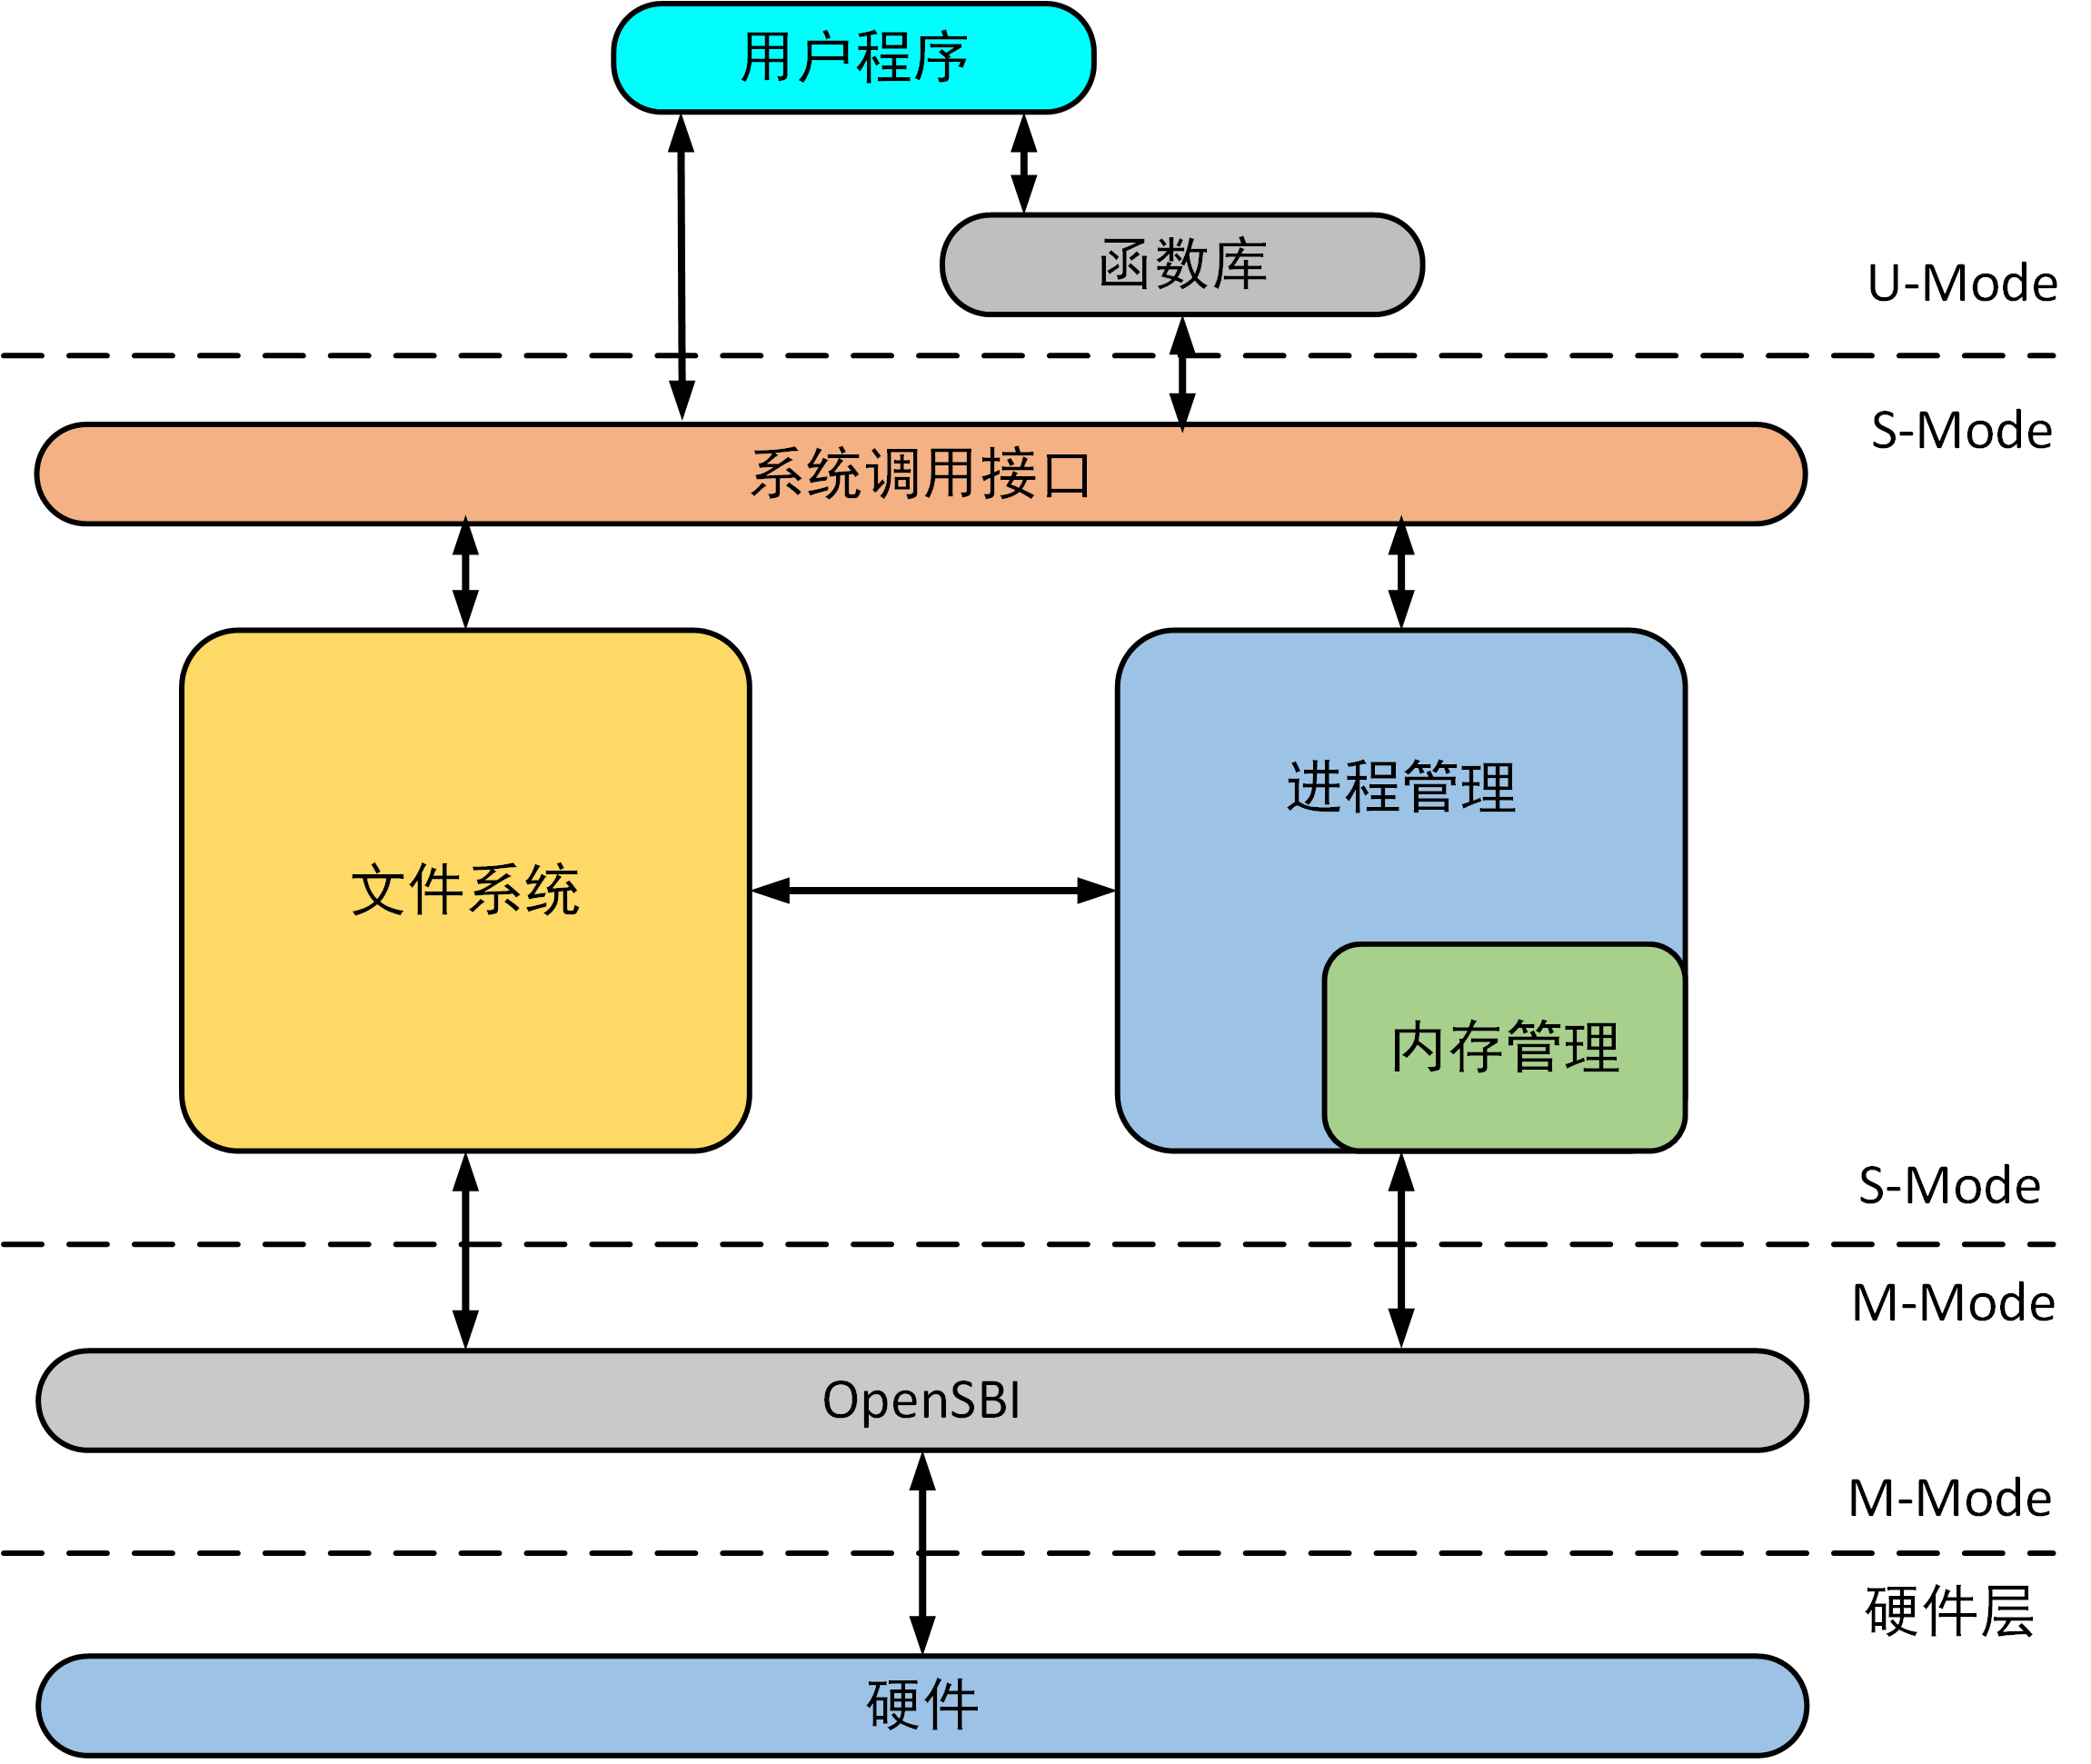
\includegraphics[width=0.75\textwidth]{moonixtotal.png}
	\setlength{\abovecaptionskip}{2pt}
	\caption{Moonix体系结构}
	\label{pic:moonixtotal}
\end{figure}

中断处理模块用于控制操作系统对内外部中断的响应。操作系统通过响应定时器中断,来定时检查进程的运行状态,可以说中断处理是进程调度的基础。内存管理模块主要通过虚拟内存管理的方式,保证各个进程能够安全共享物理内存,互不干扰。同时,由于各个进程都运行在独立的虚拟内存空间中,实现程序时不必考虑实际的物理内存状态,降低了应用程序的实现难度。进程调度模块用来控制一个进程是否可以占用CPU运行,通过Round-Robin算法\cite{DBLP:journals/eor/RasmussenT08},来保证各个进程都有相同的机会来执行代码。文件系统模块提供了一个通用的文件接口,操作系统可以不用关心不同类型文件的具体实现,而进行统一的文件读写操作。

\section{系统内存结构设计}

Moonix操作系统目前只能运行在QEMU虚拟机模拟的virt计算机上\cite{qemu/virt},以OpenSBI作为SBI。因此,Moonix可管理的内存受制于virt和OpenSBI。整个virt计算机可用物理内存大小为128MB,除去OpenSBI和Moonix内核占据的内存外,其余的内存都是Moonix操作系统可以管理的内存区域。

Moonix采用RISC-V指令集架构提供的Sv39系统来对内存进行虚拟化管理。Moonix将全部的物理地址空间映射到一个512GB大小的虚拟地址空间中,并通过填充页表来对这种映射关系进行管理,CPU在进行地址解析时就可以通过页表来执行自动的地址翻译。在Moonix中,不同的进程可以拥有不同的页表,这意味着它们运行在相互隔离的虚拟地址空间中。当一个用户进程在运行时,虚拟地址空间和虚拟地址空间的布局和映射关系如图 \ref{pic:moonixmem} 所示。

\begin{figure}[htpb]
	\centering
	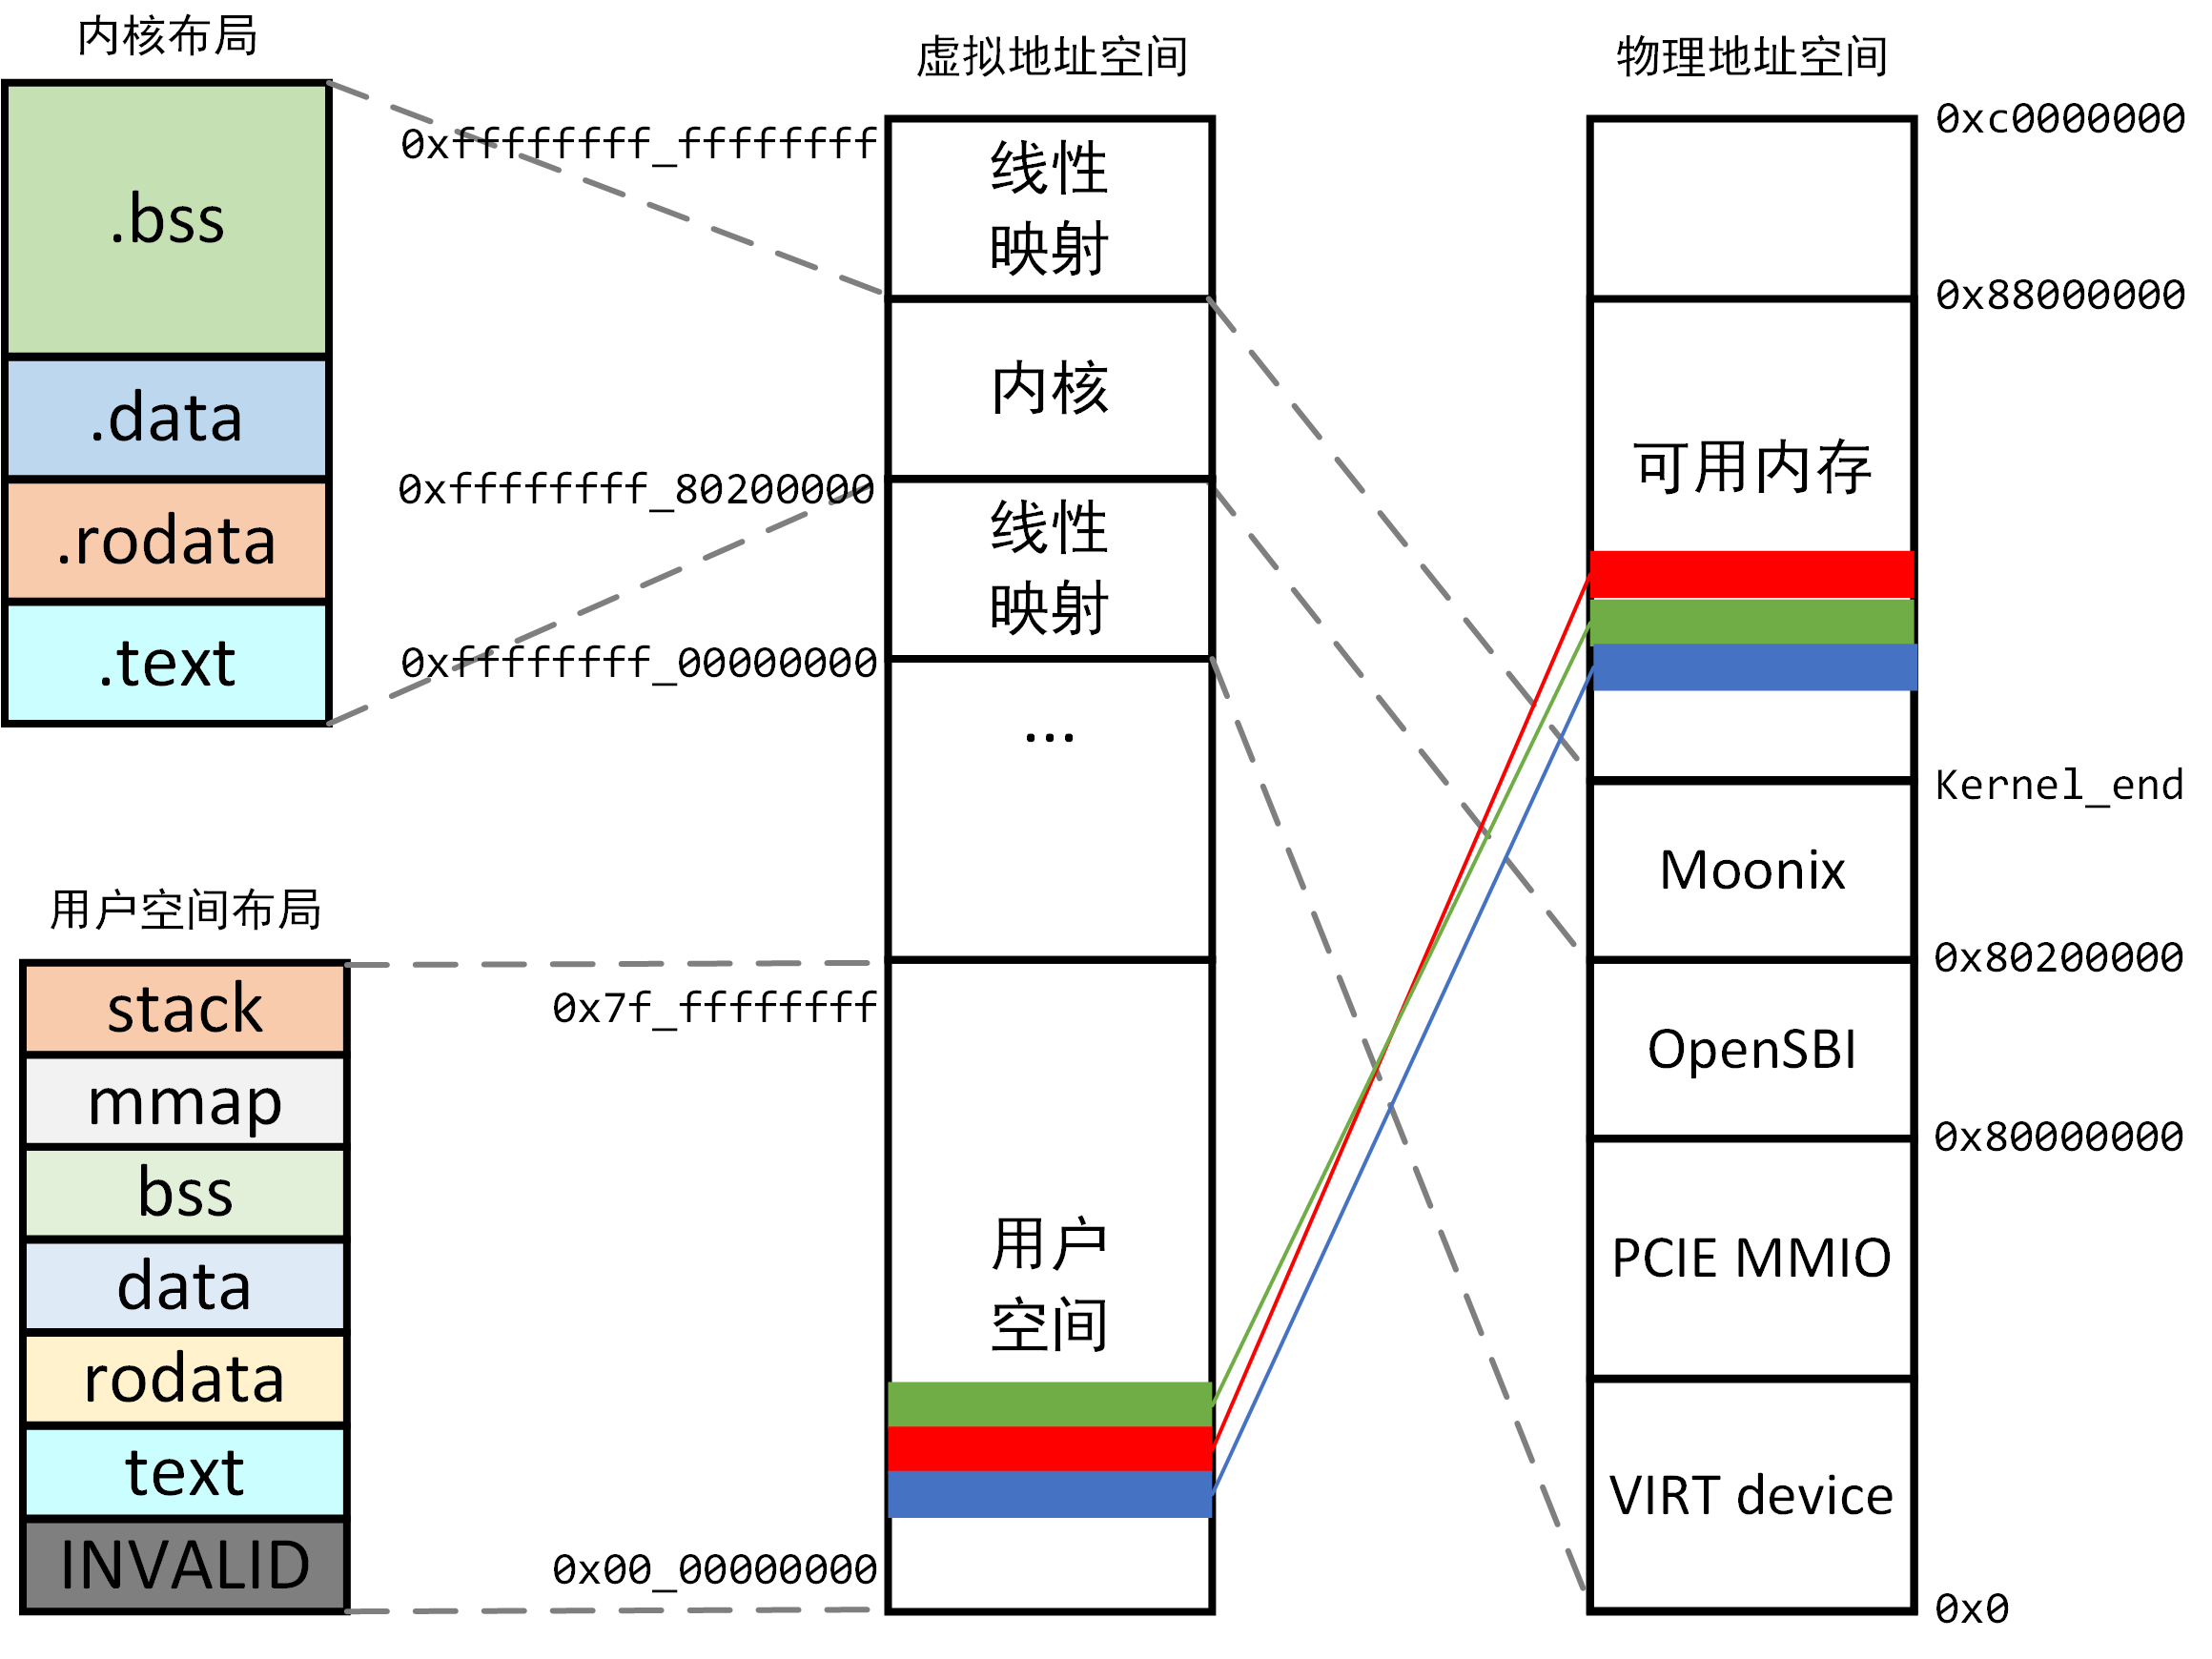
\includegraphics[width=0.85\textwidth]{mem.png}
	\setlength{\abovecaptionskip}{2pt}
	\caption{Moonix内存结构}
	\label{pic:moonixmem}
\end{figure}

在进程的虚拟地址空间中,进程的私有代码和数据占据了低地址空间,而内核的代码和数据占据了高地址空间。内核需要被映射到每个进程的高地址处,来保证用户进程在发起系统调用陷入内核时,进程能够寻找到内核的处理代码。

\section{系统内嵌的用户程序}

目前Moonix内置了两个简单的用户程序,分别是输出10遍相同字符串的hello程序,和计算并输出小于50的斐波那契数列的fib50,它们都位于文件系统上的 /bin文件夹中。

图 \ref{pic:moonixrun} 是当前Moonix操作系统的运行示例。在Moonix初始化结束之后,会输出“Welcome to Moonix!”,并启动一个可交互的shell进程。用户可以在shell中输出简单的内置命令交互,或者输入可执行文件的路径来执行程序。shell目前内置cd、ls、pwd和shutdown命令。在示例中,用户首先cd到 /bin文件夹下,运行了fib50和hello程序,接着再cd回上一级文件夹,使用相对路径的方式再次执行了一次fib50程序,最后通过shutdown命令关闭Moonix系统。

\clearpage

\begin{figure}[!h]
	%\centering
	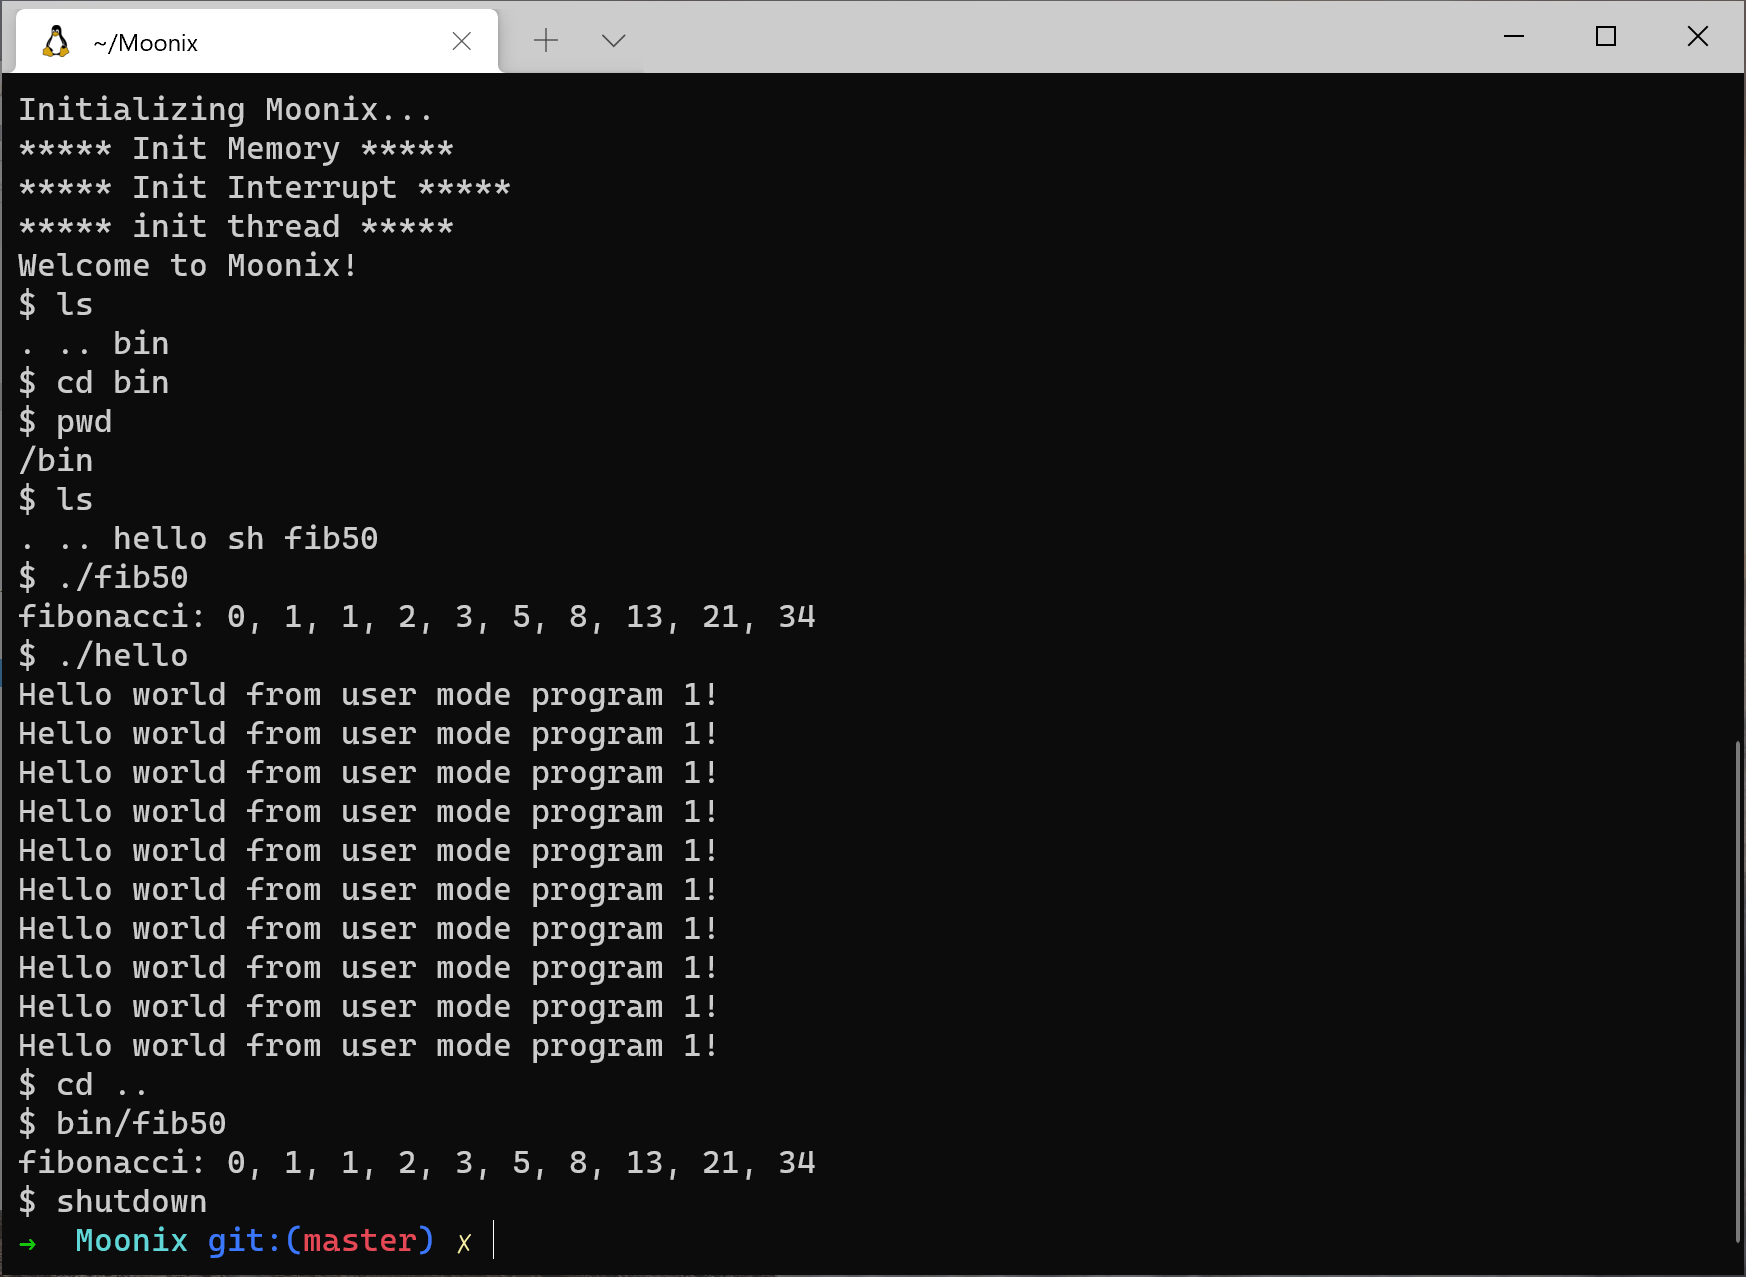
\includegraphics[width=\textwidth]{MoonixRun.png}
	%\setlength{\abovecaptionskip}{2pt}
	\caption{Moonix运行效果}
	\label{pic:moonixrun}
\end{figure}